  % ============================================================
% РОЗДІЛ 1 — переписаний (структура без підпідрозділів, стиль академічний)
% Вставити замість блоку від \protect\phantomsection\label{_Toc229682904}{}
% до \protect\phantomsection\label{_Toc228121443}{} у БКР_Тесля.tex
% ============================================================

\protect\phantomsection\label{_Toc229682904}{}РОЗДІЛ 1. АНАЛІЗ ПРЕДМЕТНОЇ
ОБЛАСТІ ТА ПОСТАНОВКА ЗАДАЧІ

\protect\phantomsection\label{_Toc229682905}{}1.1. Характеристика предметної
області

Швидке перетворення Фур'є (ШПФ, англ.~\emph{Fast Fourier Transform} ---
FFT) є одним із найбільш вживаних обчислювальних алгоритмів цифрової
обробки сигналів (ЦОС). Воно лежить в основі цифрової телекомунікації
(OFDM-модуляція у стандартах LTE, 5G, Wi-Fi), обробки мови й звуку,
радіолокації, медичного томографування, спектрального аналізу та
сучасних алгоритмів машинного навчання з перетворенням вхідних даних у
частотний простір~{[}1{]}{[}2{]}. За оцінками IEEE Signal Processing
Society, ШПФ залишається найчастіше застосовуваним числовим алгоритмом у
вбудованих системах реального часу.

Пряме обчислення дискретного перетворення Фур'є (ДПФ) має квадратичну
складність \(O(N^{2})\). Навіть для скромного розміру \(N = 1024\) це
означає понад мільйон комплексних множень, що неприйнятно для задач
реального часу. Клас швидких алгоритмів, започаткований Дж.~Кулі та
Дж.~Тюкі у 1965~р., знижує складність до \(O(N\log_{2}N)\) завдяки
рекурсивній факторизації базисної матриці {[}1{]}{[}3{]}. Для довжин, що
є степенями чотирьох (\(N = 4^{t}\)), найефективнішим з точки зору
кількості нетривіальних множень є алгоритм з основою~4 (radix-4), який
шляхом двовимірної декомпозиції зводить одновимірне ДПФ довжиною
\(N = 16\) до тристадійної схеми \(4 \times 4\): чотири паралельних
ДПФ-4, множення на матрицю поворотних множників \(W_{16}^{rk}\) та знову
чотири паралельних ДПФ-4~{[}4{]}. Алгоритм radix-4 для \(N = 16\)
потребує лише 9~нетривіальних комплексних множень проти 256~у прямому
ДПФ, що дає прискорення у 28~разів.

Паралельна природа алгоритму природно вкладається у парадигму обчислень
під керуванням потоку даних (англ.~\emph{dataflow computing}),
теоретичні засади якої були закладені Дж.~Деннісом (Jack B.~Dennis) у
MIT на початку 1970-х~рр.~{[}5{]}{[}6{]}. У dataflow-моделі відсутній
лічильник команд фон-нейманівської архітектури: вузол графа активується
тоді і лише тоді, коли на всіх його вхідних каналах є токени, після чого
самопланування системи (англ.~\emph{self-scheduling}) забезпечує
максимальний паралелізм без явних механізмів синхронізації~{[}7{]}.
Граф алгоритму ШПФ, що формально є орієнтованим ациклічним графом
залежностей за даними, відображається на граф потоку даних
(англ.~\emph{Data Flow Graph} --- DFG) без перетворення моделі.

Незважаючи на фундаментальну роль ШПФ та широкий спектр його виробничих
реалізацій, у навчальній та дослідницькій практиці існує системна
прогалина між трьома рівнями опису алгоритму. Перший рівень ---
\emph{математична модель} --- охоплює матричні факторизації, формули
метеликів і поворотних множників, що подаються у класичних підручниках із
ЦОС (Nussbaumer 1982; Burrus and Parks 1985). Другий рівень ---
\emph{формальна потокова модель} --- DFG і Synchronous Dataflow (SDF) Лі
та Месершмітта, що описують вузли, дуги, токени та правило
активації~{[}1{]}{[}4{]}. Третій рівень --- \emph{виробнича реалізація}
--- бібліотеки FFTW, ARM~CMSIS-DSP, NVIDIA~CuFFT, SPIRAL, Intel~IPP,
оптимізовані виключно під максимальну продуктивність на конкретних
платформах~{[}8{]}{[}9{]}{[}10{]}{[}11{]}{[}12{]}. Ці рівні існують
відокремлено один від одного: математичні формули не мають виконуваного
аналога з можливістю поточного спостереження; формальна SDF-модель рідко
реалізується як самостійний артефакт; а виробничі бібліотеки не надають
жодних засобів для інтерактивного дослідження внутрішньої потокової
природи алгоритму --- процесу породження та поглинання токенів, динаміки
завантаження вузлів, часу наскрізної затримки та паралельних шляхів у
графі.

Актуальність розробки візуального симулятора потокового обчислювача ШПФ
зумовлена трьома чинниками: (1)~зростанням попиту на навчальні засоби з
інтерактивною візуалізацією обчислювальних процесів у підготовці
ІТ-фахівців; (2)~розширенням інтересу до dataflow- й потокових
архітектур у сучасних спеціалізованих прискорювачах, зокрема тензорних
процесорах і FPGA-рішеннях для ЦОС; (3)~відсутністю вітчизняних
веб-орієнтованих інструментів із відкритим кодом для цього класу задач.

\protect\phantomsection\label{_Toc229682906}{}1.2. Огляд сучасних підходів та рішень

Аналіз актуальних програмних рішень і профільних літературних джерел
показує, що простір засобів обчислення ШПФ поділяється на три сегменти:
(а)~програмні бібліотеки загального призначення; (б)~апаратні та
GPU-прискорювачі; (в)~системи автоматичної генерації оптимізованого
коду. Паралельно існує окрема галузь методів візуального моделювання,
які застосовуються для формалізованого опису обчислювачів, однак не
реалізуються як виконувані симулятори. Нижче розглядаються обидва ці
напрямки.

\textbf{Бібліотека FFTW (Fastest Fourier Transform in the West)}
розроблена М.~Фріго і С.~Джонсоном у MIT у 1997~р. і у 1999~р.
відзначена премією Вілкінсона {[}13{]}. Архітектура FFTW ґрунтується на
трьох компонентах: \emph{коделети} --- компактні блоки прямолінійного
C-коду для ДПФ невеликих розмірів, автоматично згенеровані компілятором
\texttt{genfft}; \emph{планувальник} --- runtime-компонент, що методом
динамічного програмування добирає оптимальну рекурсивну факторизацію під
конкретну апаратну платформу; \emph{екзекутор} --- виконує складений
план через явну рекурсію «розділяй і володарюй». Рекурсивна декомпозиція
є кеш-незалежною (cache-oblivious): щойно підзадача поміщається у
L1/L2-кеш, вона виконується без промахів кешу, що і забезпечує вищу
продуктивність проти ітеративних реалізацій~{[}8{]}.

\textbf{ARM CMSIS-DSP} --- стандартизований пакет ЦОС для
мікроконтролерів ARM Cortex-M~{[}9{]}. Надає жорстко оптимізовані
реалізації radix-4 для розмірів \(N = 16, 64, 256, 1024, 4096\) із
ручною адаптацією під SIMD-інструкції NEON і DSP-розширення
Cortex-M4/M7. Бібліотека не переноситься на інші архітектури, не
підтримує адаптивного планування та не надає будь-яких засобів
моніторингу стану обчислення. \textbf{NVIDIA CuFFT} та \textbf{OpenCL
FFT} --- адаптації ШПФ для графічних процесорів. Стандарт OpenCL
забезпечує функціональну портативність, але не гарантує продуктивності:
ядро, оптимізоване під архітектуру NVIDIA~Fermi, демонструє низьку
ефективність на GPU ATI~Radeon через відмінності в ієрархії пам'яті та
механізмах планування потоків~{[}10{]}. Для подолання цього
застосовується автотюнінг: А.~Нукада та С.~Мацуока показали, що
адаптивний вибір відступів у спільній пам'яті та кількості активних
блоків потоків дозволяє перевершити навіть вендорну бібліотеку
NVIDIA~CuFFT {[}14{]}.

\textbf{SPIRAL} (Carnegie Mellon University) --- принципово інший
підхід: замість вибору між готовими ядрами, SPIRAL генерує
платформо-залежний код безпосередньо з математичних формул факторизації,
описаних мовою SPL (Signal Processing Language). Пошук оптимального
графа зводиться до задачі пошуку у просторі еквівалентних матричних
розкладів, що може вирішуватися евристично або методами машинного
навчання~{[}11{]}. SPIRAL генерує код як для CPU (SIMD, AVX), так і для
FPGA. \textbf{Intel IPP (Integrated Performance Primitives)} займає
проміжне місце: жорстко оптимізовані примітиви ШПФ під векторні
інструкції SSE/AVX/AVX-512 процесорів Intel без автоматичного пошуку
факторизації під час виконання~{[}12{]}.

Окрему групу джерел утворюють методи візуального моделювання, які
теоретично описують структуру обчислювачів, але не реалізуються як
виконувані симулятори з числовою верифікацією. Загальні нотації ---
UML~Activity, IDEF0/IDEF3, DFD Йордана/ДеМарко --- орієнтовані на
control-flow парадигму~{[}15{]}{[}16{]} і не мають формальної семантики
токенів, тому для потокового обчислювача ШПФ породжують надлишкові
конструкції \texttt{fork}/\texttt{join}. DFG/SDF (Data Flow Graph і
Synchronous Dataflow) --- спеціалізовані моделі для задач ЦОС, де
кількість токенів, що споживаються та виробляються кожним вузлом за одну
активацію, є фіксованою і відомою на етапі статичного аналізу~{[}7{]}{[}17{]}{[}18{]}.
Це дозволяє виконувати статичне планування без ризику взаємних блокувань
та перевіряти консистентність графа алгебраїчно через топологічну
матрицю~{[}19{]}. Алгоритм ШПФ із фіксованою довжиною \(N = 16\) є
природним прикладом SDF-графа. С.~С.~Буррус формалізує зв'язок між
матричною факторизацією та графом алгоритму через рівняння
\(\mathbf{X}' = \mathbf{C} \cdot \mathbf{D} \cdot \mathbf{A} \cdot
\mathbf{X}\), де кожна матриця відповідає окремому ярусу графа~(Burrus
and Parks 1985). Ці діаграми є статичними і не моделюють динаміку
виконання. У вітчизняній науковій традиції аналогічний підхід
застосовувався у роботах ОКБ~ЕІВТ (М.~Розенблат, 1970-ті~рр.) та у
монографії М.~М.~Яцимірського (1997~р.); зокрема, у
Фізико-механічному інституті ім.~Г.~В.~Карпенка НАН~України в 1980-х
роках було розроблено векторний спецпроцесор ШПФ на основі
dataflow-парадигми~{[}2{]}.

Узагальнення розглянутих джерел дозволяє зафіксувати три ключові
прогалини. По-перше, виробничі бібліотеки (FFTW, CMSIS-DSP, CuFFT,
SPIRAL, Intel~IPP) оптимізовані під продуктивність і не надають жодних
інтроспективних засобів: FFTW розкриває план факторизації лише у
текстовому форматі, жодна з бібліотек не генерує анімований DFG і не
показує рух токенів. По-друге, теоретичні моделі DFG/SDF формально
визначені, проте рідко супроводжуються веб-доступним симулятором із
числовою верифікацією. По-третє, статичні засоби (draw.io, Visio,
Simulink) або не відтворюють динаміки, або потребують комерційних
ліцензій, що обмежує відтворюваність у навчальному та дослідницькому
контекстах.

Порівняльна характеристика розглянутих рішень за ключовими
параметрами наведена у табл.~1.1.

Таблиця 1.1.

Порівняння існуючих рішень для обчислення ШПФ

\begin{longtable}[]{@{}
  >{\centering\arraybackslash}p{(\linewidth - 10\tabcolsep) * \real{0.1664}}
  >{\centering\arraybackslash}p{(\linewidth - 10\tabcolsep) * \real{0.1365}}
  >{\centering\arraybackslash}p{(\linewidth - 10\tabcolsep) * \real{0.2124}}
  >{\centering\arraybackslash}p{(\linewidth - 10\tabcolsep) * \real{0.1668}}
  >{\centering\arraybackslash}p{(\linewidth - 10\tabcolsep) * \real{0.1518}}
  >{\centering\arraybackslash}p{(\linewidth - 10\tabcolsep) * \real{0.1661}}@{}}
\caption[Порівняння існуючих рішень для обчислення ШПФ]{Порівняння
існуючих рішень для обчислення ШПФ}\tabularnewline
\toprule\noalign{}
\begin{minipage}[b]{\linewidth}\centering
\textbf{Рішення}
\end{minipage} & \begin{minipage}[b]{\linewidth}\centering
\textbf{Тип}
\end{minipage} & \begin{minipage}[b]{\linewidth}\centering
\textbf{Платформа}
\end{minipage} & \begin{minipage}[b]{\linewidth}\centering
\textbf{Динамічна візуалізація}
\end{minipage} & \begin{minipage}[b]{\linewidth}\centering
\textbf{Відкритий доступ}
\end{minipage} & \begin{minipage}[b]{\linewidth}\centering
\textbf{Ключова особливість}
\end{minipage} \\
\midrule\noalign{}
\endfirsthead
\toprule\noalign{}
\begin{minipage}[b]{\linewidth}\centering
\textbf{Рішення}
\end{minipage} & \begin{minipage}[b]{\linewidth}\centering
\textbf{Тип}
\end{minipage} & \begin{minipage}[b]{\linewidth}\centering
\textbf{Платформа}
\end{minipage} & \begin{minipage}[b]{\linewidth}\centering
\textbf{Динамічна візуалізація}
\end{minipage} & \begin{minipage}[b]{\linewidth}\centering
\textbf{Відкритий доступ}
\end{minipage} & \begin{minipage}[b]{\linewidth}\centering
\textbf{Ключова особливість}
\end{minipage} \\
\midrule\noalign{}
\endhead
\bottomrule\noalign{}
\endlastfoot
\textbf{1} & \textbf{2} & \textbf{3} & \textbf{4} & \textbf{5} &
\textbf{6} \\
FFTW 3.x & SW бібліотека & CPU (x86, ARM) & Немає & Так & Адаптивний
planner, cache-oblivious рекурсія~(Frigo and Johnson 2005) \\
\multicolumn{6}{@{}>{\raggedleft\arraybackslash}p{(\linewidth - 10\tabcolsep) * \real{1.0000} + 10\tabcolsep}@{}}{%
\textbf{Продовження табл. 1.1.}} \\
\textbf{1} & \textbf{2} & \textbf{3} & \textbf{4} & \textbf{5} &
\textbf{6} \\
ARM CMSIS-DSP & SW бібліотека & ARM Cortex-M & Немає & Так & Фіксований
radix-4, SIMD-оптимізація~(ARM Limited 2023) \\
NVIDIA CuFFT & SW бібліотека & GPU (NVIDIA) & Немає & Ні & Масовий
паралелізм, вендор-лок~(Du et al. 2012) \\
Nukada autotuner & SW + автотюнінг & GPU (CUDA) & Немає & Част. &
Runtime-компіляція~(Nukada and Matsuoka 2009) \\
SPIRAL & Генератор коду & CPU / FPGA & Немає & Так & Пошук у просторі
факторизацій SPL~(Püschel et al. 2004) \\
Intel IPP & SW бібліотека & Intel x86 & Немає & Ні & Примітиви
AVX/SIMD~(Intel Corporation 2021) \\
MATLAB Simulink (SDF) & Середовище моделювання & Desktop & Часткова & Ні
& SDF-модель, комерційна ліцензія \\
draw.io / Visio & Діаграмний редактор & Desktop / Web & Ні (статика) &
Част. & Лише статична схема DFG \\
\textbf{Симулятор (ця робота)} & Веб-застосунок & Браузер & \textbf{Так}
& \textbf{Так} & \textbf{Інтерактивний DFG + числова верифікація} \\
\end{longtable}

Як видно з таблиці, жодне з розглянутих рішень не поєднує одночасно
достовірного числового обчислення, інтерактивної візуалізації руху
токенів та веб-доступності без комерційної ліцензії. Саме ця незаповнена
ніша визначає предмет цієї роботи та обумовлює формулювання задачі у
підрозділі~1.5.

\protect\phantomsection\label{_Toc229682907}{}1.3. Системний аналіз задачі

Результати підрозд.~1.1--1.2 підтверджують наявність об'єктивного
розриву між математичною моделлю, формальним DFG/SDF-описом та
виробничими реалізаціями алгоритму ШПФ. Для структурованого опису цього
розриву та переходу до постановки задачі застосовується системний
аналіз: визначаються зацікавлені сторони, цілі розробки, обмеження та
критерії успіху.

Потенційні користувачі та бенефіціари розроблюваного симулятора наведені
у табл.~1.2.

Таблиця 1.2.

Зацiкавленi сторони та їхнi основнi потреби

\begin{longtable}[]{@{}
  >{\raggedright\arraybackslash}p{(\linewidth - 4\tabcolsep) * \real{0.2512}}
  >{\raggedright\arraybackslash}p{(\linewidth - 4\tabcolsep) * \real{0.3551}}
  >{\raggedright\arraybackslash}p{(\linewidth - 4\tabcolsep) * \real{0.3937}}@{}}
\caption[Зацікавлені сторони та їхні основні потреби]{Зацікавлені
сторони та їхні основні потреби}\tabularnewline
\toprule\noalign{}
\begin{minipage}[b]{\linewidth}\raggedright
\textbf{Сторона}
\end{minipage} & \begin{minipage}[b]{\linewidth}\raggedright
\textbf{Потреба}
\end{minipage} & \begin{minipage}[b]{\linewidth}\raggedright
\textbf{Як симулятор її задовольняє}
\end{minipage} \\
\midrule\noalign{}
\endfirsthead
\toprule\noalign{}
\begin{minipage}[b]{\linewidth}\raggedright
\textbf{Сторона}
\end{minipage} & \begin{minipage}[b]{\linewidth}\raggedright
\textbf{Потреба}
\end{minipage} & \begin{minipage}[b]{\linewidth}\raggedright
\textbf{Як симулятор її задовольняє}
\end{minipage} \\
\midrule\noalign{}
\endhead
\bottomrule\noalign{}
\endlastfoot
Студенти спеціальності 122 «Комп'ютерні науки» & Зрозуміти внутрішню
роботу алгоритму ШПФ, побачити паралелізм і токенну динаміку & Анімація
руху токенів по DFG, крок-за-кроком режим, теплова карта активності
вузлів \\
Викладачі курсів ЦОС та паралельних обчислень & Демонстраційний
інструмент для лекційних і лабораторних занять & Веб-застосунок без
встановлення, відтворюваність на будь-якій ОС \\
Дослідники dataflow-архітектур & Перевірка гіпотез щодо планування та
критичного шляху графа ШПФ & Метрики throughput/latency/queue, event
log, налаштовувані затримки \\
Інженери DSP/FPGA на ранній стадії проєктування & Попередня оцінка
потокової моделі перед апаратною реалізацією & Параметричне налаштування
\texttt{latency} і \texttt{delay}, експорт подій \\
\end{longtable}

На основі проаналізованої предметної області та потреб зацікавлених
сторін визначено ієрархію цілей. \textbf{Генеральна ціль:} створити
програмний симулятор, що відтворює потокове виконання 16-точкового
алгоритму ШПФ radix-4 \(4 \times 4\) та забезпечує його інтерактивну
графічну візуалізацію у вигляді анімованого DFG зі спостереженням
токенів, метрик і наскрізної затримки. Підцілі, що випливають із
генеральної:

\begin{itemize}
\item
  формалізувати граф потоку даних для алгоритму radix-4 \(4 \times 4\) з
  вузлами типів \texttt{source}, \texttt{dft4}, \texttt{twiddle},
  \texttt{sink} та дугами із параметричними затримками;
\item
  реалізувати ядро симуляції з правилом активації токенів, FIFO-чергами
  та керованим логічним часом;
\item
  забезпечити інтерактивну візуалізацію руху токенів, теплову карту
  активності вузлів і спектральний вихід;
\item
  виконати числову верифікацію результатів шляхом порівняння з еталонним
  обчисленням ДПФ.
\end{itemize}

Розробка виконується у таких обмеженнях. \emph{Технічні} --- цільова
платформа виконання: сучасний веб-браузер (Chrome/Firefox/Edge) з
підтримкою JavaScript ES2020; відсутність серверної частини (повністю
клієнтська симуляція). \emph{Ресурсні} --- розробка силами одного
виконавця у межах бакалаврської кваліфікаційної роботи. \emph{Часові}
--- термін виконання згідно з календарним графіком кафедри.
\emph{Алгоритмічні} --- фіксований розмір перетворення \(N = 16\) як
базовий демонстраційний розмір; розширення на довільні \(N = 4^{t}\)
залишається напрямком подальшого розвитку. \emph{Правові} ---
використання лише програмних бібліотек з відкритими ліцензіями (MIT,
Apache~2.0, BSD) без комерційних компонентів.

Результат роботи вважається досягнутим, якщо одночасно виконуються такі
вимірювані критерії: максимальне відхилення вихідного спектра симулятора
від еталонного ДПФ за модулем не перевищує \(\varepsilon = 10^{- 9}\);
чотири вузли \texttt{dft4} першого ярусу виконуються паралельно, що
підтверджується одночасними подіями \texttt{onFire} у журналі симуляції;
користувач може керувати швидкістю симуляції у діапазоні не менш ніж
\(0.1 \times\)~--~\(4 \times\) без втрати коректності; час відгуку
інтерфейсу на користувацькі дії (пуск, пауза, зміна швидкості) не
перевищує 100~мс.

\protect\phantomsection\label{_Toc229682908}{}1.4. Етичні, правові та
регуляторні аспекти

Розроблюваний симулятор працює лише із синтетичними тестовими сигналами,
що формуються або вводяться користувачем у межах локального сеансу
роботи. Система не опрацьовує персональних, медичних, біометричних чи
фінансових даних, не передає інформацію на зовнішні сервери та не
використовує моделі штучного інтелекту для автоматизованого ухвалення
рішень. Тому вимоги GDPR і Закону України «Про захист персональних
даних» мають для цього проєкту обмежену прикладну релевантність, однак
базові принципи мінімізації даних, прозорості опрацювання та відсутності
прихованого збору інформації все одно дотримуються.

З регуляторного погляду для роботи суттєвими є насамперед вимоги до
якості програмного забезпечення, коректності числових обчислень та
оформлення результатів. У цьому контексті враховано положення
ISO/IEC\textasciitilde{}25010 щодо функціональної придатності,
продуктивності та зручності використання, стандарт
IEEE\textasciitilde{}754 щодо подання чисел з плаваючою крапкою, а також
ДСТУ\textasciitilde{}3008:2015 і
ДСТУ\textasciitilde{}ГОСТ\textasciitilde{}7.1:2006, які регламентують
оформлення пояснювальної записки та списку використаних джерел. Окремо
дотримується принцип академічної доброчесності: усі зовнішні джерела та
референтні реалізації належно процитовані, а отримані результати є
відтворюваними.

\protect\phantomsection\label{_Toc229682909}{}1.5. Постановка задачі та
формулювання вимог

Нехай задано комплекснозначну вхідну послідовність
\(\{ x_{n}\}_{n = 0}^{N - 1}\) довжиною \(N = 16\), подану у подвійній
точності формату IEEE~754. Потрібно розробити програмний симулятор,
який: (1)~обчислює дискретне перетворення Фур'є

\[X_{k} = \sum_{n = 0}^{N - 1}x_{n}\, e^{- j2\pi nk/N},\quad k = 0,1,\ldots,N - 1,\]

за алгоритмом radix-4 з двовимірною \(4 \times 4\) декомпозицією,
реалізованим у моделі потоку даних; (2)~подає процес обчислення у
вигляді орієнтованого графа потоку даних \(G = (V,E)\), де \(V\) ---
множина операцій, а \(E\) --- множина спрямованих зв'язків між ними;
(3)~виконує симуляцію графа з дотриманням правила активації (вузол
спрацьовує тоді і лише тоді, коли на всіх його вхідних каналах є
токени) та з урахуванням часових параметрів виконання операцій і
передавання даних; (4)~забезпечує інтерактивну візуалізацію процесу
обчислення та подає кінцевий спектр \(\{ X_{k}\}\) у вигляді
амплітудної діаграми.

\textbf{Вхідні дані симулятора:} послідовність
\(\{ x_{n}\}_{n = 0}^{15}\) --- 16~комплексних відліків сигналу,
задається користувачем або генерується вбудованим джерелом (синусоїда,
одиничний імпульс, білий шум); параметри симуляції --- часові
характеристики обробки, параметри передавання даних між операціями та
множник швидкості відтворення; команди керування --- пуск, пауза,
покроковий режим, скидання стану. \textbf{Вихідні дані симулятора:}
спектр \(\{ X_{k}\}_{k = 0}^{15}\) --- 16~комплексних відліків, що
візуалізуються як амплітуда \(|X_{k}|\) і фаза \(\arg X_{k}\); журнал
подій --- часові мітки надходження даних, активації операцій і
формування результатів; метрики роботи графа --- пропускна здатність
(throughput), наскрізна затримка (latency), розмір черг (queue size),
теплова карта активності вузлів; звіт про верифікацію --- максимальне
відхилення \(\max_{k}|X_{k}^{sim} - X_{k}^{ref}|\) відносно еталонного
ДПФ.

Функціональні вимоги до симулятора зведено у табл.~1.3.

Таблиця 1.3.

Функціональні вимоги до симулятора

\begin{longtable}[]{@{}
  >{\centering\arraybackslash}p{(\linewidth - 4\tabcolsep) * \real{0.0517}}
  >{\centering\arraybackslash}p{(\linewidth - 4\tabcolsep) * \real{0.2332}}
  >{\centering\arraybackslash}p{(\linewidth - 4\tabcolsep) * \real{0.7130}}@{}}
\caption[Функціональні вимоги до симулятора]{Функціональні вимоги до
симулятора}\tabularnewline
\toprule\noalign{}
\begin{minipage}[b]{\linewidth}\raggedright
\textbf{ID}
\end{minipage} & \begin{minipage}[b]{\linewidth}\raggedright
\textbf{Назва}
\end{minipage} & \begin{minipage}[b]{\linewidth}\raggedright
\textbf{Опис}
\end{minipage} \\
\midrule\noalign{}
\endfirsthead
\toprule\noalign{}
\begin{minipage}[b]{\linewidth}\raggedright
\textbf{ID}
\end{minipage} & \begin{minipage}[b]{\linewidth}\raggedright
\textbf{Назва}
\end{minipage} & \begin{minipage}[b]{\linewidth}\raggedright
\textbf{Опис}
\end{minipage} \\
\midrule\noalign{}
\endhead
\bottomrule\noalign{}
\endlastfoot
\textbf{1} & \textbf{2} & \textbf{3} \\
F1 & Побудова DFG & Автоматична генерація графа потоку даних для ШПФ
radix-4 \(4 \times 4\) при \(N = 16\) \\
F2 & Симуляція виконання & Крокування часу з доставкою токенів,
перевіркою правила активації та виконанням вузлів \\
F3 & Введення сигналу & Вибір типу вхідного сигналу (синусоїда, імпульс,
шум) та його параметрів \\
\multicolumn{3}{@{}>{\raggedleft\arraybackslash}p{(\linewidth - 4\tabcolsep) * \real{0.9980} + 4\tabcolsep}@{}}{%
\textbf{Продовження табл. 1.3.}} \\
\textbf{1} & \textbf{2} & \textbf{3} \\
F4 & Керування симуляцією & Пуск, пауза, покроковий режим, скидання,
зміна множника швидкості \\
F5 & Візуалізація токенів & Анімоване переміщення токенів по дугах з
відображенням значень \\
F6 & Відображення метрик & Показ throughput, latency, queue size,
теплової карти активності \\
F7 & Спектральний вихід & Відображення амплітуди та фази \(\{ X_{k}\}\)
у вигляді гістограми \\
F8 & Верифікація результату & Порівняння з еталонним ДПФ і виведення
максимального відхилення \\
F9 & Налаштування параметрів & Редагування часових параметрів моделі без
перезавантаження сторінки \\
\end{longtable}

Нефункціональні вимоги регламентують якісні характеристики системи у
відповідності до ISO/IEC~25010 (табл.~1.4).

Таблиця 1.4.

Нефункціональні вимоги до симулятора

\begin{longtable}[]{@{}
  >{\raggedright\arraybackslash}p{(\linewidth - 4\tabcolsep) * \real{0.0689}}
  >{\raggedright\arraybackslash}p{(\linewidth - 4\tabcolsep) * \real{0.3027}}
  >{\raggedright\arraybackslash}p{(\linewidth - 4\tabcolsep) * \real{0.6219}}@{}}
\caption[Нефункціональні вимоги до симулятора]{Нефункціональні вимоги до
симулятора}\tabularnewline
\toprule\noalign{}
\begin{minipage}[b]{\linewidth}\raggedright
\textbf{ID}
\end{minipage} & \begin{minipage}[b]{\linewidth}\raggedright
\textbf{Характеристика}
\end{minipage} & \begin{minipage}[b]{\linewidth}\raggedright
\textbf{Вимога}
\end{minipage} \\
\midrule\noalign{}
\endfirsthead
\toprule\noalign{}
\begin{minipage}[b]{\linewidth}\raggedright
\textbf{ID}
\end{minipage} & \begin{minipage}[b]{\linewidth}\raggedright
\textbf{Характеристика}
\end{minipage} & \begin{minipage}[b]{\linewidth}\raggedright
\textbf{Вимога}
\end{minipage} \\
\midrule\noalign{}
\endhead
\bottomrule\noalign{}
\endlastfoot
NF1 & Точність обчислень &
\(\max_{k}|X_{k}^{sim} - X_{k}^{ref}| \leq 10^{- 9}\) \\
NF2 & Час відгуку UI & Реакція на користувацьку дію \(\leq 100\)~мс \\
NF3 & Частота кадрів & Стабільні 60~fps при швидкості симуляції
\(\leq 5 \times\) \\
NF4 & Портативність & Коректна робота у сучасних поширених
веб-браузерах \\
NF5 & Детермінованість & Однаковий вхід і параметри дають ідентичний
журнал подій \\
NF6 & Відкритий код & Розповсюдження під ліцензією MIT або Apache~2.0 \\
NF7 & Без встановлення & Робота у браузері без серверної частини та
БД \\
NF8 & Зручність & Основні операції доступні не глибше двох кліків від
головного екрану \\
\end{longtable}

У системі виділяються два актори --- \emph{Студент} (первинний
користувач, спостерігач) і \emph{Викладач} (вторинний користувач, може
налаштовувати сценарії демонстрації). Графічне подання прецедентів
наведено на рис.~1.1, а їхній деталізований перелік --- у табл.~1.5.

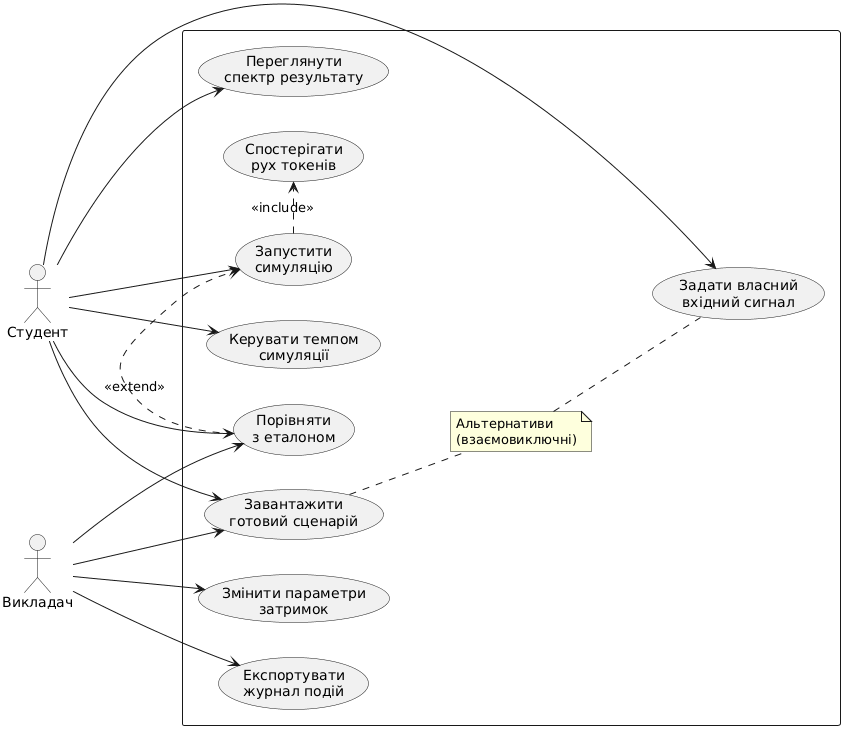
\includegraphics[width=6.49583in,height=5.62153in]{media/media/image1.png}

Рис. 1.1. Use Case-діаграма симулятора потокового обчислювача ШПФ

На діаграмі показано, що UC3 містить (include) UC5, а UC7 розширює
(extend) UC3. Прецеденти UC1 і UC2 є взаємовиключними альтернативами
підготовки вхідних даних.

Таблиця 1.5.

Перелік прецедентів (Use Cases) симулятора

\begin{longtable}[]{@{}
  >{\raggedright\arraybackslash}p{(\linewidth - 6\tabcolsep) * \real{0.0717}}
  >{\raggedright\arraybackslash}p{(\linewidth - 6\tabcolsep) * \real{0.2622}}
  >{\raggedright\arraybackslash}p{(\linewidth - 6\tabcolsep) * \real{0.1748}}
  >{\raggedright\arraybackslash}p{(\linewidth - 6\tabcolsep) * \real{0.4913}}@{}}
\caption[Перелік прецедентів (Use Cases) симулятора]{Перелік прецедентів
(Use Cases) симулятора}\tabularnewline
\toprule\noalign{}
\begin{minipage}[b]{\linewidth}\raggedright
\textbf{ID}
\end{minipage} & \begin{minipage}[b]{\linewidth}\raggedright
\textbf{Прецедент}
\end{minipage} & \begin{minipage}[b]{\linewidth}\raggedright
\textbf{Актор}
\end{minipage} & \begin{minipage}[b]{\linewidth}\raggedright
\textbf{Стислий опис}
\end{minipage} \\
\midrule\noalign{}
\endfirsthead
\toprule\noalign{}
\begin{minipage}[b]{\linewidth}\raggedright
\textbf{ID}
\end{minipage} & \begin{minipage}[b]{\linewidth}\raggedright
\textbf{Прецедент}
\end{minipage} & \begin{minipage}[b]{\linewidth}\raggedright
\textbf{Актор}
\end{minipage} & \begin{minipage}[b]{\linewidth}\raggedright
\textbf{Стислий опис}
\end{minipage} \\
\midrule\noalign{}
\endhead
\bottomrule\noalign{}
\endlastfoot
UC1 & Завантажити готовий сценарій & Студент, Викладач & Обрати один із
передустановлених входів (синусоїда, імпульс, шум) \\
UC2 & Задати власний вхідний сигнал & Студент & Ввести 16~комплексних
відліків вручну \\
UC3 & Запустити симуляцію & Студент & Ініціювати виконання DFG з пуску
до завершення \\
UC4 & Керувати темпом симуляції & Студент & Пауза, step-by-step, зміна
множника швидкості \\
UC5 & Спостерігати рух токенів & Студент & Переглядати анімацію токенів
по дугах у реальному часі \\
UC6 & Переглянути спектр результату & Студент & Побачити \(|X_{k}|\) і
\(\arg X_{k}\) у вигляді діаграми \\
UC7 & Порівняти з еталоном & Студент, Викладач & Виконати зіставлення з
референтним обчисленням і побачити похибку \\
UC8 & Змінити параметри затримок & Викладач & Налаштувати часові
характеристики вузлів і зв'язків графа \\
UC9 & Експортувати журнал подій & Викладач & Зберегти журнал подій у
файл для подальшого аналізу \\
\end{longtable}

\emph{Підпорядкування прецедентів:} UC3 містить (\emph{include}) UC5
(рух токенів автоматично супроводжує виконання); UC7 розширює
(\emph{extend}) UC3 та може бути викликаний після завершення симуляції;
UC1 і UC2 є взаємовиключними альтернативами підготовки вхідних даних.
Описана постановка задачі та перелік вимог утворюють технічне завдання,
яке далі конкретизується у розділі~2 через вибір методів і технологій
реалізації, проєктування архітектури та структур даних.

\protect\phantomsection\label{_Toc229682910}{}1.6. Висновки до розділу~1

У першому розділі виконано аналіз предметної області, огляд сучасних
підходів, системний аналіз задачі, розгляд етичних та правових аспектів
і формалізовано постановку задачі.

Зафіксовано \emph{стан предметної області:} алгоритм ШПФ radix-4
\(4 \times 4\) для \(N = 16\) має достатньо розроблений математичний
апарат і формальні потокові моделі (DFG, SDF), однак у практичному
інструментарії ці рівні описані відокремлено. Виробничі бібліотеки
(FFTW, ARM~CMSIS-DSP, NVIDIA~CuFFT, SPIRAL, Intel~IPP) оптимізовані
виключно для продуктивності та не надають засобів інтроспекції. Методи
візуального моделювання (UML, IDEF0, DFG/SDF, сигнальні графи)
залишаються переважно теоретичними та не реалізуються як інтерактивні
веб-симулятори з числовою верифікацією.

Виявлено \emph{прогалину:} жодне з розглянутих рішень не поєднує
одночасно достовірного обчислення ШПФ за формальною SDF-моделлю,
інтерактивної динамічної візуалізації руху токенів і веб-доступності без
комерційної ліцензії. Саме ця незаповнена ніша визначає предмет цієї
роботи.

Сформульовано \emph{задачу} розробки програмного симулятора потокового
обчислювача 16-точкового ШПФ з анімованим DFG, визначено вхідні та
вихідні дані, технічні, ресурсні й правові обмеження та критерії успіху.
Розроблено перелік із 9~функціональних (F1--F9) і 8~нефункціональних
(NF1--NF8) вимог, побудовано перелік із 9~прецедентів (UC1--UC9), що
охоплюють основні сценарії використання симулятора студентами та
викладачами. Ключові вимірювані критерії --- точність
\(\varepsilon \leq 10^{- 9}\), час відгуку \(\leq 100\)~мс, стабільні
60~fps при швидкості до \(3 \times\) --- підлягають експериментальній
перевірці у розділі~4.

Розглянуто етичні та правові аспекти: робота не опрацьовує персональних
даних, базується на відкритих ліцензіях (MIT, Apache~2.0) і відповідає
стандартам ISO/IEC~25010, IEEE~754, ECMAScript~2020, ДСТУ~3008:2015 та
ДСТУ~ГОСТ~7.1:2006. Математичне та алгоритмічне обґрунтування (виведення
формул radix-4 \(4 \times 4\), матричні факторизації, формалізація
DFG/SDF) виноситься до розділу~2, де воно подається у складі проєктного
обґрунтування обраних методів і архітектури системи.